\documentclass[a4paper, 12pt]{article}
\usepackage[portuges]{babel}
\usepackage[utf8]{inputenc}
\usepackage{amsmath, amssymb}
\usepackage{indentfirst}
\usepackage{graphicx}
\usepackage{geometry}
\geometry{a4paper, top=2.5cm, bottom=2.5cm, left=2.5cm, right=2.5cm}
\usepackage{booktabs}
\usepackage{tabularx}
\usepackage{multirow}
\usepackage{array}
\usepackage{caption}
\usepackage{fancyhdr}
\usepackage[hidelinks]{hyperref}
\usepackage{float}
\usepackage{ragged2e}

% Configurações para tabularx
\newcolumntype{Y}{>{\raggedright\arraybackslash}X}
\newcolumntype{Z}{>{\centering\arraybackslash}X}

\pagestyle{fancy}
\fancyhf{}
\rhead{Projeto de Rede Corporativa - BRL}
\lhead{}
\rfoot{Página \thepage}

\begin{document}

\begin{titlepage}
    \begin{center}
        \vspace*{1cm}
        {\Large{\textbf{Projeto de Rede Corporativa}}}\\
        \vspace{0.8cm}
        {\large{\textbf{Empresa BRL}}}\\
        \vspace{1.2cm}
        
\includegraphics[width=0.3\textwidth]{pucpr.png}
        \vspace{1.2cm}
        
        \begin{flushleft}
            \begin{tabbing}
                \hspace{3cm} \= \kill
                \textbf{Integrantes:} \\
                \> Renan da Silva Oliveira Andrade \\
                \> Leticia Maria Maia de Andrade Vieira \\
                \> Brenda Gabrielli Barbosa \\
                \\
                \textbf{Orientador:} \\
                \> Prof. Dr. Ricardo Cassiano Nabhen \\
            \end{tabbing}
        \end{flushleft}
        \vspace{\fill}
        \large{Outubro de 2025}
    \end{center}
\end{titlepage}

\tableofcontents
\thispagestyle{empty}
\newpage

\pagenumbering{arabic}

\section{Apresentação do Projeto}
\label{sec:apresentacao}

O projeto tem como seu principal objetivo o design e implementação de uma rede corporativa de campus para a empresa BRL. A rede conectará duas localidades, a Matriz localizada em São Paulo e a Filial localizada em Curitiba, por meio de uma conexão segura através da Internet. O design hierárquico de redes será aplicado em ambos os site, dividindo a infraestrutura em camadas lógicas pensadas para otimizar o desempenho, a segurança e a escalabilidade da empresa.

\section{Objetivos do Projeto}
\label{sec:objetivos}

\begin{itemize}
    \item Implementar um design de rede hierárquico: Separar a rede em camadas de acesso, distribuição e núcleo para melhor gerenciamento e desempenho.
    \item Garantir conectividade segura e redundante: Estabelecer uma conexão principal via VPN sobre a Internet e um link de backup para assegurar a continuidade do serviço entre os dois sites.
    \item Segregar o tráfego de rede: Utilizar VLANs para criar redes independentes para os dois departamentos em cada site, mantendo a interconectividade.
    \item Centralizar serviços corporativos: Consolidar serviços essenciais como VoIP, DNS e web no datacenter da Matriz.
    \item Assegurar alta disponibilidade e segurança: Implementar regras de firewall e NAT/NAPT para controlar o acesso à Internet e proteger a rede interna contra ameaças externas.
\end{itemize}

\section{Descrição do Cenário de Rede}
\label{sec:descricao}

A empresa BRL opera em duas unidades: a Matriz (São Paulo) com 150 usuários, e a Filial (Curitiba) com 100 usuários. Em ambos os sites, a rede interna é segmentada em dois departamentos. Havendo participantes de ambos os departamentos em cada switch presente na rede.

\subsection{Aplicações e Serviços}
\label{subsec:aplicacoes}

\begin{itemize}
    \item \textbf{ERP}: Servidores em ambos os sites (HTTP).
    \item \textbf{DNS}: Servidor hospedado na Matriz responsável pelos sites, www.brl.com.br (Matriz) e www.brlfilial.com.br (Filial).
    \item \textbf{Telefonia IP (VoIP)}: Utiliza o protocolo SIP (UDP 5060, 5061) e RTP (UDP 10000-11000) para comunicação interna e entre as unidades. Há um servidor VoIP no datacenter de cada site.
    \item \textbf{Acesso à Internet}: O tráfego de saída dos usuários é restrito aos serviços HTTP, HTTPS, DNS e ICMP (ping).
\end{itemize}

\section{Projeto Lógico da Rede}
\label{sec:projeto-logico}

\subsection{Topologia da Rede}
\label{subsec:topologia}

\begin{figure}[H]
    \centering
    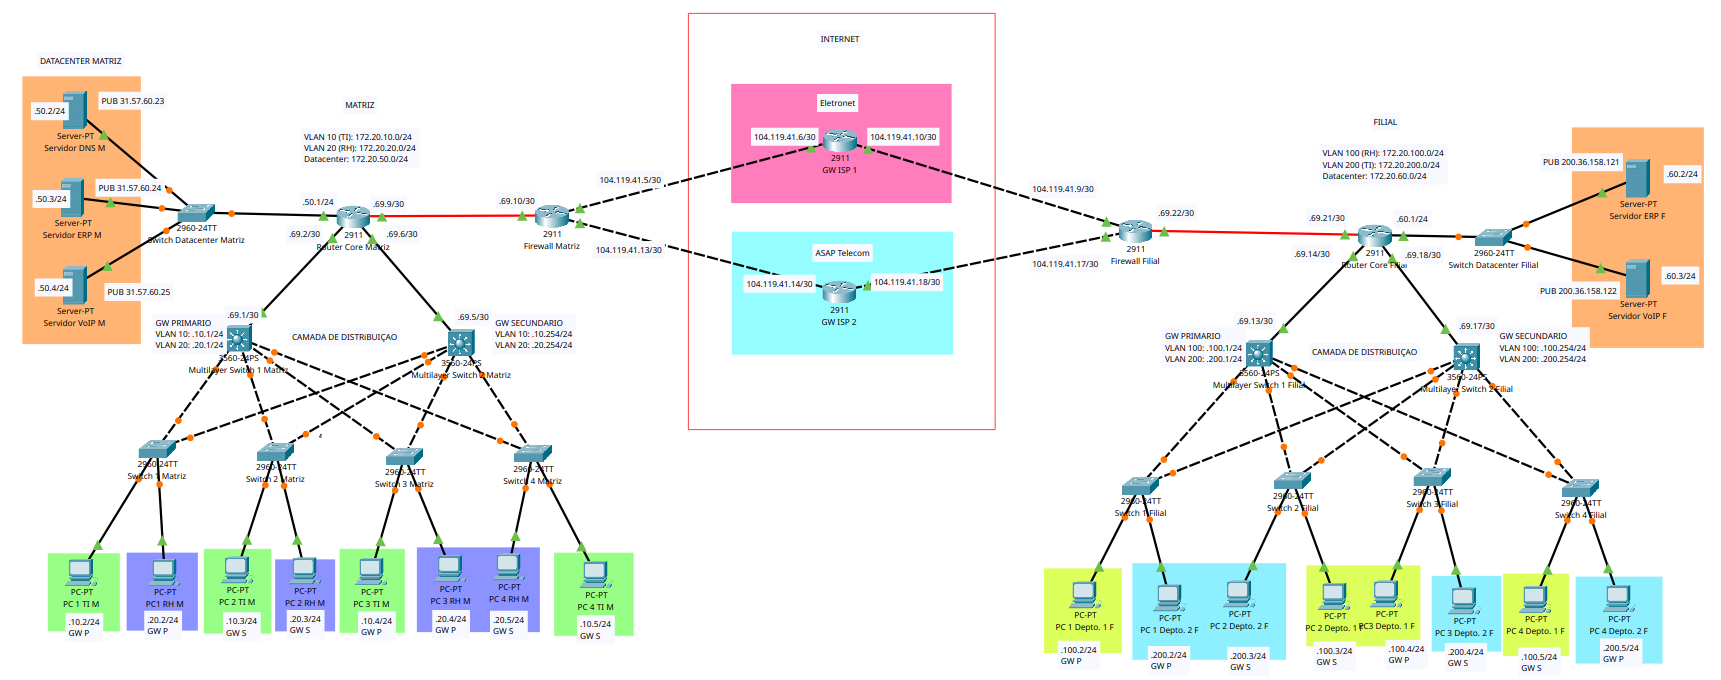
\includegraphics[width=1\linewidth]{geral.png}
        \caption{Diagrama Geral das Topologias das Redes}
    \label{fig:geral}
\end{figure}

A topologia foi implementada no modelo hierárquico de três camadas (Núcleo, Distribuição e Acesso) em ambos os sites (Matriz e Filial). A conectividade entre os sites é garantida por um enlace VPN Site-to-Site sobre a Internet, com links redundantes para provedores de serviços.

\begin{figure}[H]
    \centering
    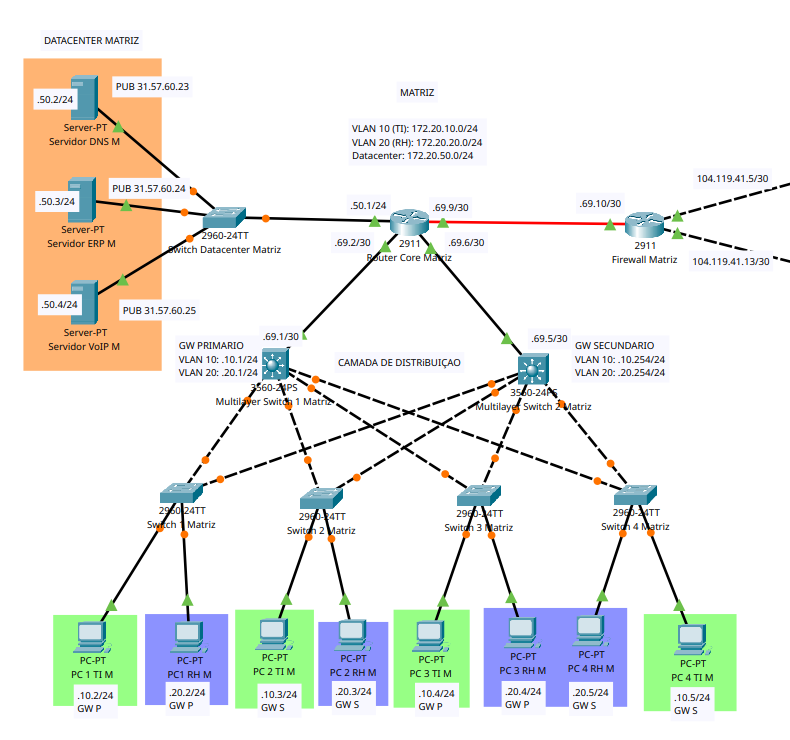
\includegraphics[width=0.8\linewidth]{matriz.png}
    \caption{Diagrama da Topologia das Redes da Matriz}
    \label{fig:matriz}
\end{figure}

No diagrama da topologia da matriz, estão presentes 6 redes IPs: 1 rede IP designada ao data center, 2 redes IPs destinadas às VLANs (10 e 20), 2 redes ponto-a-ponto conectando os Multilayer Switches ao Roteador Core, e uma rede ponto-a-ponto conectando o Roteador Core ao Firewall.

Podemos identificar na topologia da rede as seguintes camadas do modelo hierárquico, onde os 4 Switches 2960-24TT representam a \textbf{Camada de Acesso}, que é a responsável por conectar os dispositivos de ponta à LAN.

Acima deles, estão posicionados 2 Multilayer Switches 3560-24PS, que compõem a \textbf{Camada de Distribuição}. Todos os switches da Camada de Acesso estão propositalmente conectados aos dois multilayer switches, para fornecer a redundância de link, distribuindo o acesso à rede.

Acima dos multilayer switches, está posicionado um Roteador 2911, responsável pela \textbf{Camada de Núcleo}, que tem como objetivo interconectar todos os dispositivos entre as LANs, entre si e às redes externas.

Em laranja, temos uma rede IP dedicada ao Data Center. Onde os servidores se conectam a um switch 2960-24TT, responsável por conectá-los ao roteador Core. Além de segregar as redes LAN da rede do data center, os servidores possuem acesso direto ao link de mais alta velocidade da rede.

Por último, temos um roteador segregado que aplica as \textbf{Regras de Firewall}, ele também é o Gateway Padrão do roteador core, e age como roteador de borda da rede, fornecendo conectividade à WAN.

Todos os aspectos topológicos comentados acima, podem ser visualizados na Figura \ref{fig:matriz}.

\begin{figure}[H]
    \centering
    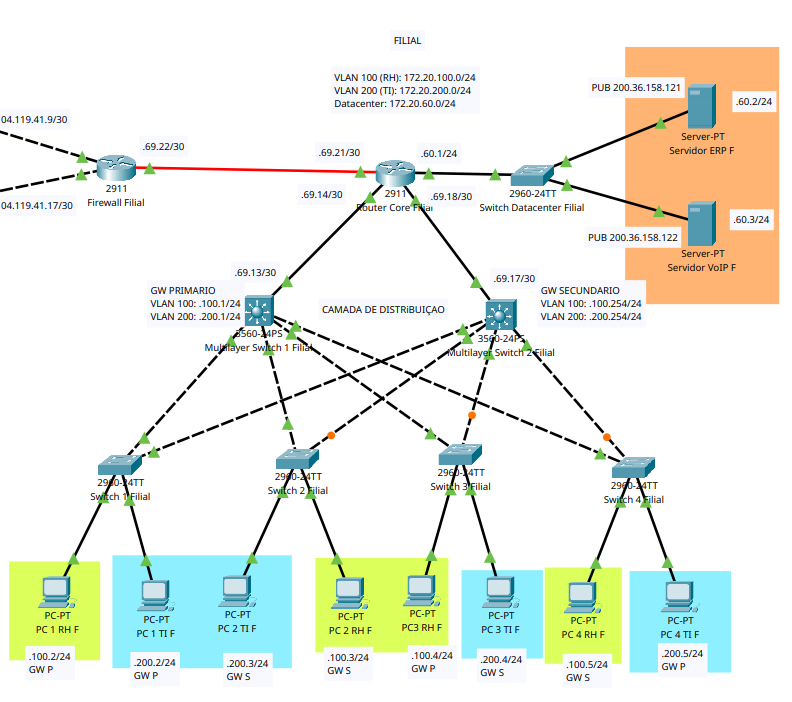
\includegraphics[width=0.8\linewidth]{filial.png}
    \caption{Diagrama da Topologia das Redes da Filial}
    \label{fig:filial}
\end{figure}

A topologia da rede Filial é um espelho da rede Matriz, com a única exceção de conter um servidor a menos (servidor DNS), conforme demonstrado na Figura \ref{fig:filial}. 

\begin{figure}[H]
    \centering
    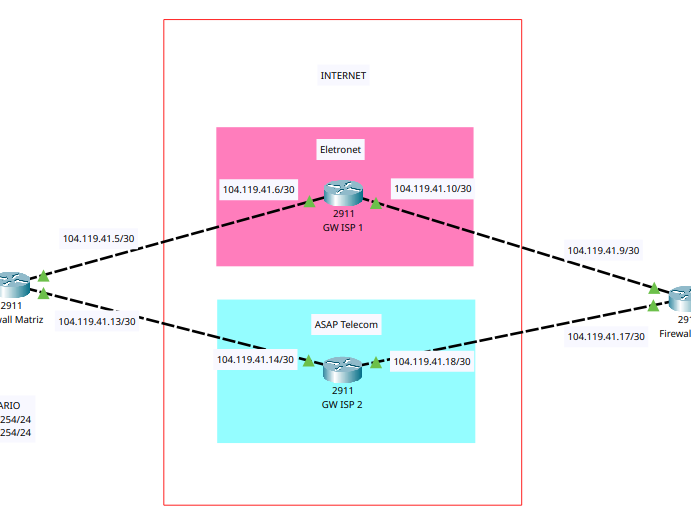
\includegraphics[width=0.8\linewidth]{isp.png}
    \caption{Diagrama da Topologia das ISPs}
    \label{fig:isp}
\end{figure}

Para fins de redundância, o cenário leva em conta, a contratação de dois Provedores de Serviço de Internet (ISPs). Conforme observado na Figura \ref{fig:isp}, os dois ISPs são representados por dois roteadores distintos, que realizam o intermédio entre os dois sites Matriz e Filial, e (não demonstrado aqui) a conectividade à Internet. Os roteadores de borda de cada site (roteadores de firewall), se conectam diretamente ao roteador do provedor, estabelecendo assim a conexão dos sites à redes externas.

\subsection{Divisão de VLANs e Esquema de Endereçamento IP}
\label{subsec:vlan}

A segregação de tráfego é realizada através de VLANs, conforme detalhado na Tabela  \ref{tab:vlans}.

\begin{table}[H]
\centering
\caption{Esquema de VLANs e Endereçamento IP}
\label{tab:vlans}
\begin{tabularx}{\textwidth}{YYYYY}
\toprule
\textbf{Local} & \textbf{VLAN} & \textbf{Sub-rede} & \textbf{GW Primário} & \textbf{GW Secundário} \\
\midrule
Matriz & TI (VLAN 10) & 172.20.10.0/24 & 172.20.10.1 & 172.20.10.254 \\
Matriz & RH (VLAN 20) & 172.20.20.0/24 & 172.20.20.1 & 172.20.20.254 \\
Filial & RH (VLAN 100) & 172.20.100.0/24 & 172.20.100.1 & 172.20.100.254 \\
Filial & TI (VLAN 200) & 172.20.200.0/24 & 172.20.200.1 & 172.20.200.254 \\
Matriz & Datacenter & 172.20.50.0/24 & 172.20.50.1 & N/A \\
Filial & Datacenter & 172.20.60.0/24 & 172.20.60.1 & N/A \\
\bottomrule
\end{tabularx}
\end{table}

Todos os VLAN IDs foram configurados nas VLAN DBs dos switches das camadas de acesso, e dos multilayer switches das camadas de distribuição de ambas matriz e filial, onde a conexão entre switches e, entre switches e roteadores está configurada em modo TRUNK, enquanto as portas dos switches das camadas de acesso que estão conectadas a dispositivos de usuários, estão configuradas em modo ACCESS com a respectiva VLAN a qual pertence.

\subsection{Endereçamento de Servidores}
\label{subsec:servidores}

Os servidores corporativos possuem endereçamento estático, com mapeamento para IPs públicos via NAT, conforme mostra a Tabela \ref{tab:servidores}.

\begin{table}[H]
\centering
\caption{Endereçamento de Servidores e NAT}
\label{tab:servidores}
\begin{tabularx}{\textwidth}{YYYY}
\toprule
\textbf{Serviço} & \textbf{Local} & \textbf{IP Privado} & \textbf{IP Público (NAT Estático)} \\
\midrule
DNS & Matriz & 172.20.50.2/24 & 31.57.60.23 \\
ERP & Matriz & 172.20.50.3/24 & 31.57.60.24 \\
VoIP & Matriz & 172.20.50.4/24 & 31.57.60.25 \\
ERP & Filial & 172.20.60.2/24 & 200.36.158.121 \\
VoIP & Filial & 172.20.60.3/24 & 200.36.158.122 \\
\bottomrule
\end{tabularx}
\end{table}

\subsection{Links Ponto-a-Ponto e IPs Públicos}
\label{subsec:links}

Todas as redes ponto-a-ponto utilizam CIDR /30. Para links ponto-a-ponto entre dispositivos internos utiliza-se a faixa 172.20.69.x/30. Os links para ISPs utilizam os seguintes endereçamentos públicos:
\begin{itemize}
    \item \textbf{Firewall Matriz $\rightarrow$ ISP Eletronet}: 104.119.41.4/30
    \item \textbf{Firewall Matriz $\rightarrow$ ISP ASAP Telecom}: 104.119.41.12/30
    \item \textbf{Firewall Filial $\rightarrow$ ISP Eletronet}: 104.119.41.8/30
    \item \textbf{Firewall Filial $\rightarrow$ ISP ASAP Telecom}: 104.119.41.16/30
\end{itemize}

Para o NAPT (NAT Overload), são utilizados os IPs próprios das portas do roteador firewall. Portanto, os IPs compartilhados por hosts das LANs (exceto os servidores) são:

\begin{itemize}
    \item \textbf{Hosts Matriz via ISP Eletronet}: 104.119.41.5/32
    \item \textbf{Hosts Matriz via ISP ASAP Telecom}: 104.119.41.13/32
    \item \textbf{Hosts Filial via ISP Eletronet}: 104.119.41.9/32
    \item \textbf{Hosts Filial via ISP ASAP Telecom}: 104.119.41.17/32
\end{itemize}


\subsection{Projeto de Roteamento}
\label{subsec:roteamento}

A redundância é alcançada através da configuração de múltiplos caminhos, e da utilização de dois provedores de Internet. O protocolo de roteamento padrão do Cisco Packet Tracer, será utilizado para a troca dinâmica de informações de rota entre os dispositivos de camada 3 (Multilayer Switches e Roteador Core), garantindo assim a convergência da rede em caso de falhas.

Ambos os Multilayer Switches possuem como rota padrão o roteador core, e conhecem as redes das duas VLANs.

Já o roteador core, conhece todas as redes internas, incluindo as redes diretamente conectadas (redes do data center e do firewall), e rotas estáticas para as redes das VLANs, tendo como rota padrão o firewall (roteador de borda da rede).

O firewall conhece as redes das duas ISPs, bem como a rede ponto-a-ponto estabelecida com o roteador core. Além disso, possui também rotas estáticas para as redes VLANs, juntamente com a rede do data center.

A estratégia utilizada para estabelecer redundância de link entre o firewall e os ISPs, é estabelecer ambos os links como rotas padrão, porém estabelecendo um peso (\textit{cost}) maior no ISP de backup (ASAP Telecom), fazendo assim com que o firewall prefira o ISP principal (Eletronet) e utilize o ISP secundário em caso de falha do primeiro link.

\section{Serviços de Rede}
\label{sec:servicos}

\subsection{Configuração de NAT/NAPT}
\label{subsec:nat}

O serviço de tradução de endereços de rede (NAT) é configurado no firewall de borda para:
\begin{itemize}
    \item \textbf{NAT Estático}: Mapeamento one-to-one de IPs públicos para os servidores internos (Tabela \ref{tab:servidores}), permitindo acesso externo controlado.
    \item \textbf{PAT (NAPT Overload)}: Tradução de todos os IPs privados das VLANs de usuários para os IPs públicos das interfaces de saída do firewall, permitindo o acesso múltiplo e simultâneo à Internet.
\end{itemize}

\subsection{Regras de Firewall}
\label{subsec:firewall}

A política de segurança ``Default Deny'' é implementada, negando explicitamente todo o tráfego não permitido. As regras são baseadas no princípio do menor privilégio, garantindo a segurança da rede. 

\subsubsection{Política de Firewall Matriz}

O firewall da Matriz adota uma política de permitir comunicações essenciais entre a rede interna, a filial e serviços externos, conforme descrito:

\begin{itemize}
    \item \textbf{HTTP/HTTPS:} é permitido o tráfego de saída e entrada para navegação web segura, com portas 80 e 443.
    \item \textbf{DNS:} consultas DNS são liberadas tanto para saída quanto para retorno de respostas, utilizando UDP na porta 53
    \item \textbf{ICMP:} pacotes ICMP são autorizados para permitir testes de conectividade (ping) entre as redes internas e externas.
    \item \textbf{ERP:} comunicação bidirecional entre o servidor ERP da Matriz (172.20.50.3) e os IPs de clientes da Filial de ambas as ISPs, com portas 80 e 443 para aplicação.
    \item \textbf{DNS Interno:} é permitido o acesso de IPs de clientes da Filial ao servidor DNS interno da Matriz para resolução de nomes internos (brl.com.br e brlfilial.com.br).
    \item \textbf{SIP/RTP (Voz sobre IP):} é permitido o tráfego de voz (SIP nas portas 5060–5061 e RTP entre 10000–11000) entre o servidor VoIP da Matriz e o servidor VoIP da filial (200.36.158.122), garantindo comunicação VoIP exclusiva entre os dois sites.
\end{itemize}.

\begin{figure}
    \centering
    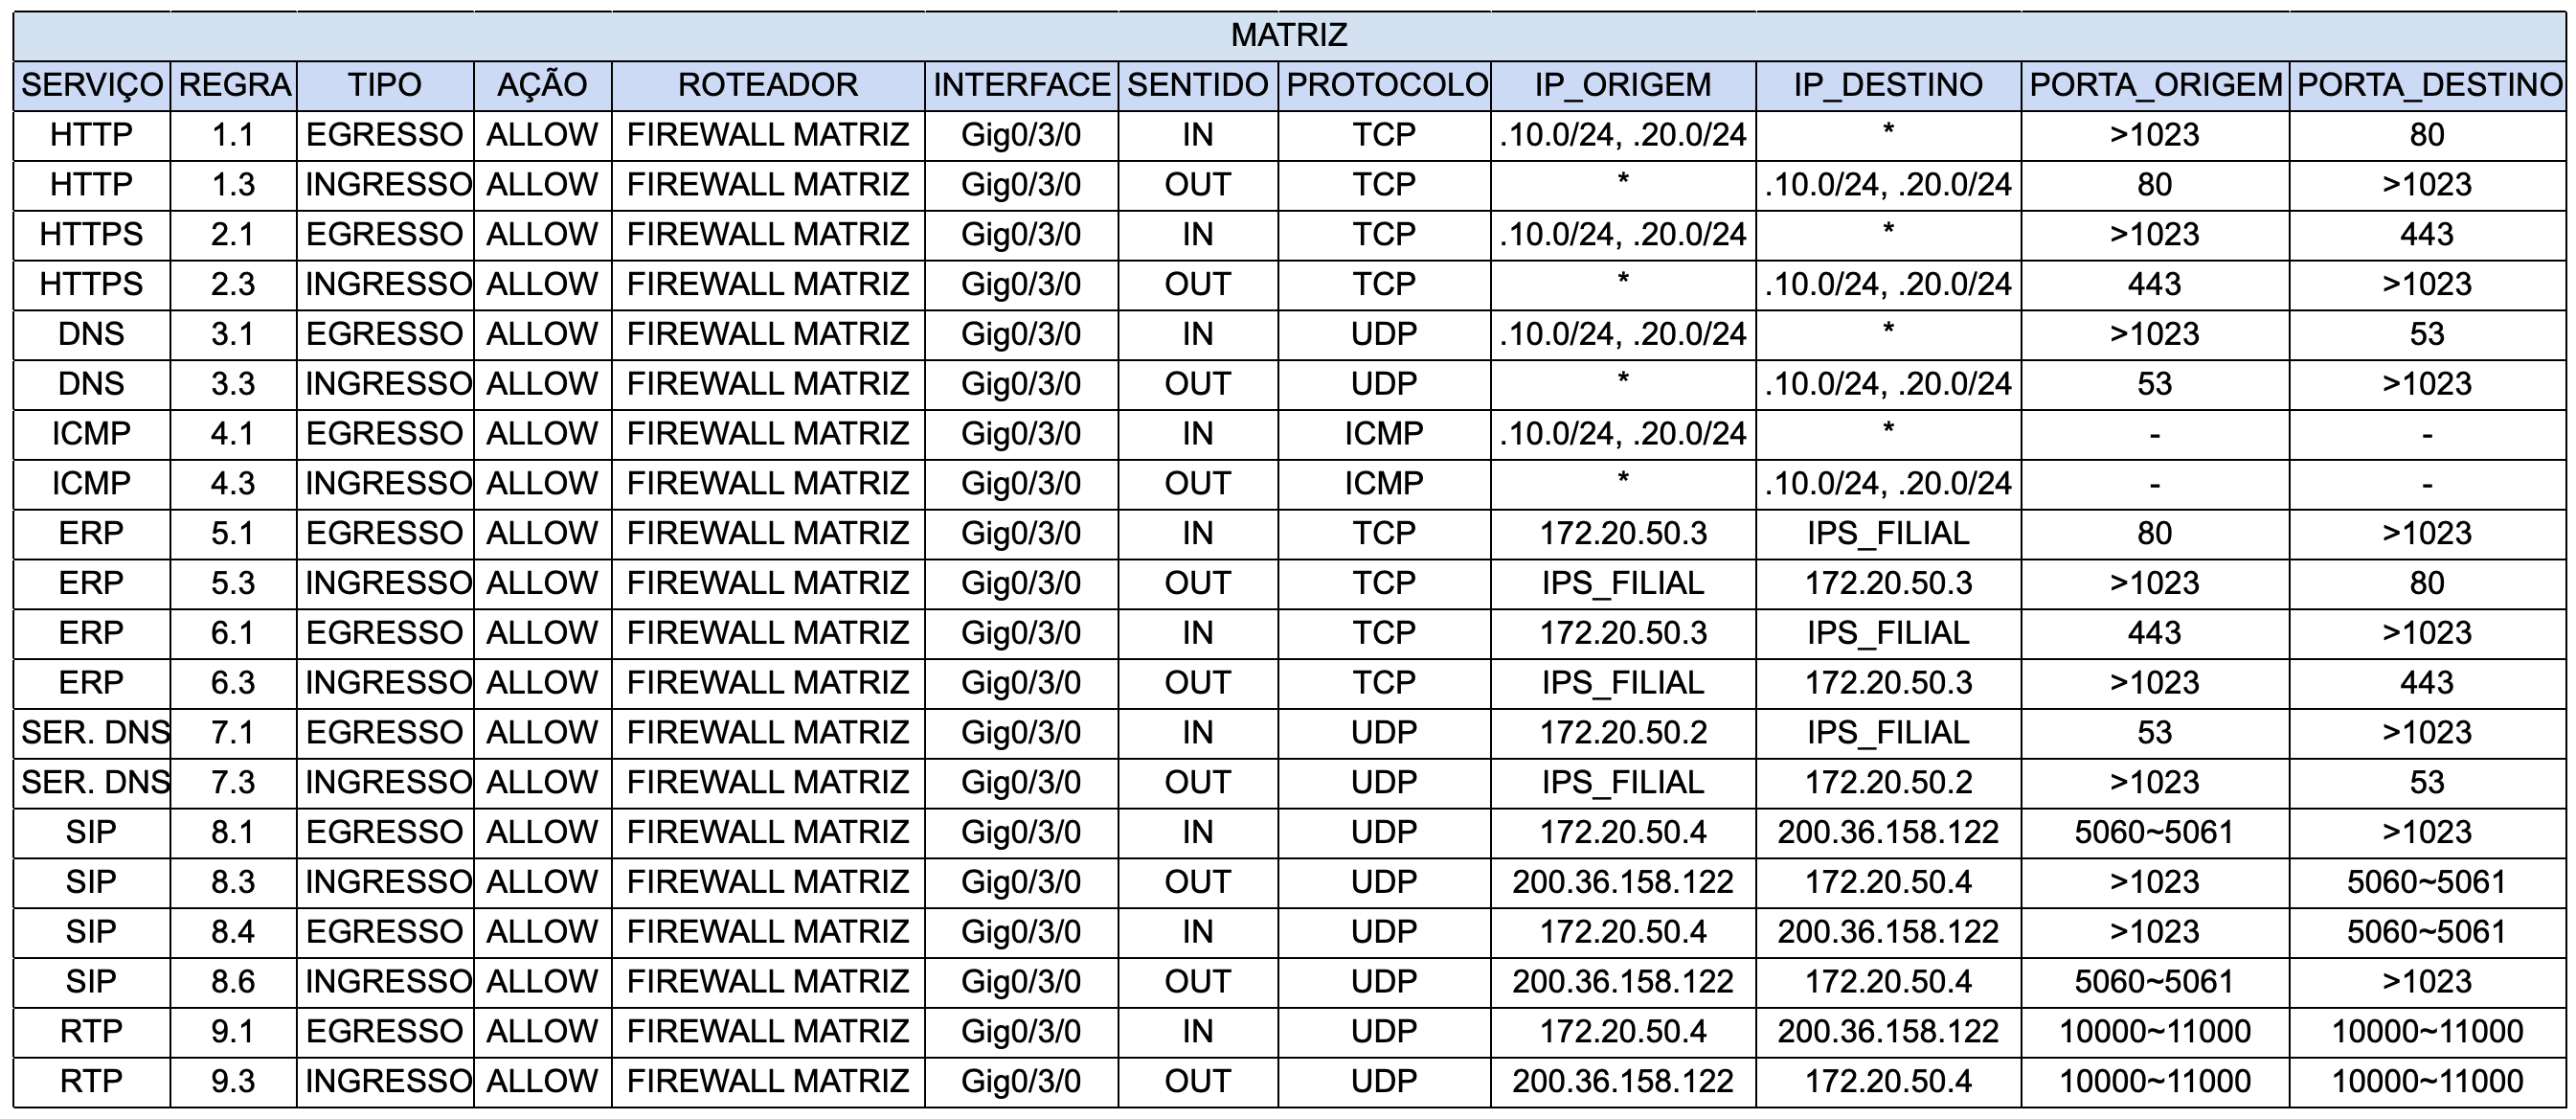
\includegraphics[width=1\linewidth]{tabela-matriz.png}
    \caption{Regras de Firewall - Matriz}
    \label{fig:placeholder}
\end{figure}

Em resumo, a Matriz atua como ponto principal da rede corporativa, controlando fluxos com a filial e o provedor VoIP, e liberando serviços web, DNS e ERP de forma controlada.

\subsubsection{Política de Firewall Filial}

O firewall da Filial segue uma política espelhada, com foco em acesso controlado à Matriz e à Internet:

\begin{itemize}
    \item \textbf{HTTP/HTTPS:} libera acesso web de saída e retorno de respostas para toda a rede local (100.0/24, 200.0/24).
    \item \textbf{DNS:} permite consultas e respostas DNS via UDP, tanto internas quanto externas.
    \item \textbf{ICMP:} autoriza pacotes ICMP para verificação de conectividade.
    \item \textbf{ERP:} garante comunicação segura entre o servidor ERP da Filial (172.20.60.2) e os hosts da Matriz, nas portas 80 e 443, para sincronização e acesso de dados e de sistemas corporativos.
    \item \textbf{SIP/RTP:} permite comunicação de voz entre o servidor VoIP da Filial (172.20.60.3) e o servidor VoIP da Matriz (31.57.60.25), estabelecendo uma conexão bidirecional exclusiva entre Matriz e Filial.
\end{itemize}

Assim, a Filial mantém conectividade segura com a Matriz e com a Internet, restringindo o tráfego apenas a protocolos e portas estritamente necessárias.

\begin{figure}
    \centering
    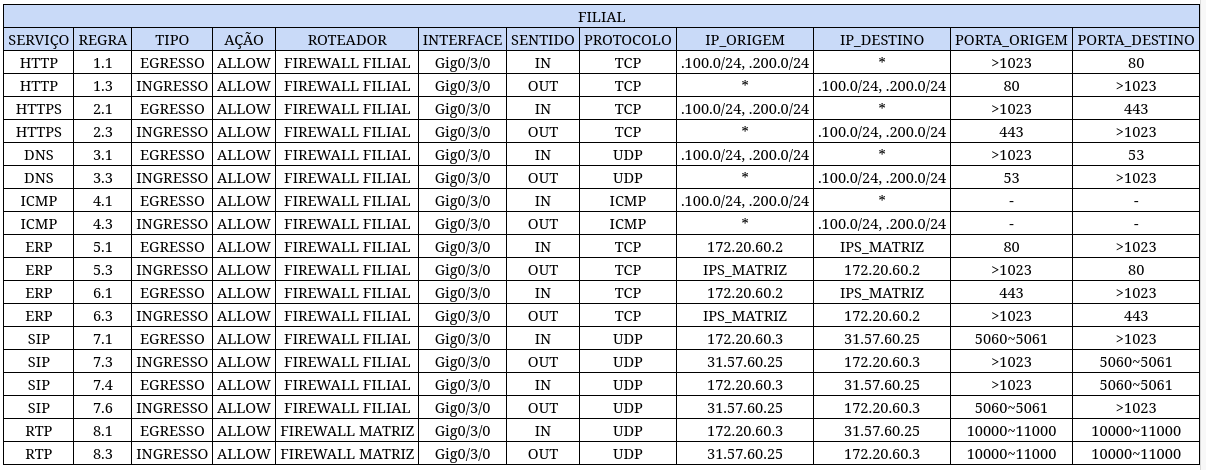
\includegraphics[width=1\linewidth]{tabela-filial.png}
    \caption{Regras de Firewall - Filial}
    \label{fig:placeholder}
\end{figure}

\subsection{Especificações do Link de Internet e SLA}
\label{subsec:provedores}

Para garantir conectividade robusta e em conformidade com as necessidades empresariais, foram selecionados dois provedores de telecomunicações com atuação nacional e reconhecida qualidade em links corporativos de alta disponibilidade: \textbf{Eletronet} e \textbf{ASAP Telecom}. As principais características dos serviços estão resumidas na Tabela \ref{tab:provedores}.

\begin{table}[H]
\centering
\caption{Especificações dos Provedores de Internet}
\label{tab:provedores}
\begin{tabularx}{\textwidth}{YYY}
\toprule
\textbf{Provedor / Serviço} & \textbf{Largura de Banda} & \textbf{SLA (Acordo de Nível de Serviço)} \\
\midrule
\textbf{Eletronet (Principal)} & Link Dedicado IP Corporativo – até 400 Gbps (Fibra Óptica DWDM) & Disponibilidade de 99,95\%, latência média nacional $<$15 ms, suporte 24x7, tempo de reparo $<$4h \\[4pt]
\textbf{ASAP Telecom (Backup)} & Link Dedicado de Internet – até 10 Gbps (Fibra Óptica ponto a ponto) & Disponibilidade de 99,5\%, latência média nacional $<$25 ms, suporte 24x7, tempo de reparo $<$6h \\
\bottomrule
\end{tabularx}
\end{table}

O \textit{Service Level Agreement} (SLA) define os parâmetros de desempenho e disponibilidade contratados com os provedores. O serviço da Eletronet \cite{eletronet} utiliza rede óptica baseada em tecnologia \textit{DWDM} (Dense Wavelength Division Multiplexing), com backbone próprio de mais de 17 mil km interligando os principais pontos de troca de tráfego (PTTs) do Brasil, permitindo conexões de até 400~Gbps com baixa latência e suporte corporativo contínuo. 

Já o serviço da ASAP Telecom \cite{asap} é implementado sobre fibra óptica dedicada (\textit{link ponto a ponto}), oferecendo redundância ao link principal com banda contratual de até 10~Gbps, gerenciamento proativo de falhas e monitoramento em tempo real.

O SLA de 99,95\% ofertado pela Eletronet implica em até cerca de 4h22min de indisponibilidade anual, enquanto o SLA de 99,5\% da ASAP Telecom representa até 1 dia e 19h de possível inatividade ao ano — valores aceitáveis dentro de um cenário de contingência empresarial. 

As métricas de desempenho incluem latência, \textit{packet loss}, tempo de resolução de falhas e disponibilidade contínua do serviço, elementos essenciais para a estabilidade de aplicações críticas como ERP, VPN e VoIP.

\subsection{Especificações da VPN Site-to-Site}
\label{subsec:vpn}

Para garantir a comunicação segura entre a Matriz e a Filial, interligadas por meio de provedores de Internet distintos e potencialmente inseguros, é proposta a implementação de uma \textbf{VPN (Virtual Private Network)} no modelo Site-to-Site utilizando o protocolo IPSec em modo túnel. 

Essa abordagem permite encapsular e criptografar todo o tráfego IP entre as duas redes locais corporativas, garantindo confidencialidade, integridade e autenticação ponta a ponta entre os roteadores/firewalls de borda de ambas as unidades.

\subsubsection{Arquitetura e Topologia de Comunicação}
\label{subsubsec:vpn-topology}

A VPN será estabelecida entre os firewalls de borda de cada localidade:
\begin{itemize}
    \item \textbf{Firewall Matriz:} IPs públicos 104.119.41.5 (Eletronet) e 104.119.41.13 (ASAP Telecom)
    \item \textbf{Firewall Filial:} IPs públicos 104.119.41.9 (Eletronet) e 104.119.41.17 (ASAP Telecom)
\end{itemize}

Ambos os firewalls estarão configurados como \textit{peers} IPSec, estabelecendo um túnel direto através da Internet pública. Cada firewall atuará simultaneamente como gateway local para suas redes privadas internas:
\begin{itemize}
    \item Redes internas da Matriz: 172.20.10.0/24, 172.20.20.0/24, 172.20.50.0/24
    \item Redes internas da Filial: 172.20.100.0/24, 172.20.200.0/24, 172.20.60.0/24
\end{itemize}

O tráfego destinado de uma rede à outra será roteado automaticamente pelo túnel criptografado, com o firewall realizando \textit{encapsulation/decapsulation} conforme a direção do tráfego.

\subsubsection{Configurações Técnicas da VPN IPSec}
\label{subsubsec:vpn-config}

\begin{itemize}
    \item \textbf{Modo de Operação:} Túnel (Tunnel Mode).
    \item \textbf{Protocolo de Segurança:} IPSec (Internet Protocol Security).
    \item \textbf{Camada de Implementação:} Camada de Rede (Camada 3 – Modelo OSI).
    \item \textbf{Criptografia:} AES-256 GCM (Advanced Encryption Standard Galois/Counter Mode, chave de 256 bits) para proteção de dados em trânsito.
    \item \textbf{Integridade e Autenticação:} SHA-256 (Secure Hash Algorithm 256-bit) para verificação de integridade e autenticação do pacote.
    \item \textbf{Troca de Chaves:} IKEv2 (Internet Key Exchange, versão 2), utilizando Diffie-Hellman Group 14 (2048 bits).
    \item \textbf{Tempo de Vida da SA (Security Association):} 8 horas para rekeying automático.
    \item \textbf{Modo de Transporte:} ESP (Encapsulating Security Payload), operando sobre o protocolo IP (protocolo 50).
    \item \textbf{Protocolos Suportados:} Compatibilidade com \textit{OpenVPN} e \textit{L2TP/IPSec} para interoperabilidade futura.
\end{itemize}

\subsubsection{Mecanismos de Estabelecimento do Túnel}
\label{subsubsec:vpn-handshake}

O processo de inicialização do túnel ocorre em duas fases:
\begin{enumerate}
    \item \textbf{Fase 1 (IKE SA):} Estabelece um canal seguro para troca de parâmetros de autenticação e negociação das chaves criptográficas. Ambas as partes autenticam-se mutuamente via \textit{pre-shared key} (PSK) ou certificados digitais X.509.
    \item \textbf{Fase 2 (IPSec SA):} Define os parâmetros do túnel (endereços locais/remotos, algoritmos de criptografia e integridade). A partir dessa fase, o tráfego entre os sub-redes é criptografado e transmitido de forma segura.
\end{enumerate}

\subsubsection{Fluxo de Comunicação}
\label{subsubsec:vpn-flow}

O funcionamento da VPN segue a sequência abaixo:
\begin{enumerate}
    \item Um dispositivo de umas das redes da Filial (por exemplo, 172.20.10.2) envia um pacote destinado à uma das redes da Matriz (por exemplo, 172.20.100.0/24).
    \item O firewall da Filial identifica o tráfego como pertencente à política IPSec e encapsula o pacote original em um cabeçalho IPSec.
    \item O pacote criptografado é transmitido pela Internet (link da Eletronet ou ASAP Telecom) até o firewall da Matriz.
    \item O firewall da Matriz valida a integridade e autenticidade do pacote, descriptografa o conteúdo e encaminha-o internamente à rede de destino.
    \item O processo inverso ocorre para o tráfego no sentido oposto.
\end{enumerate}

\subsubsection{Redundância e Monitoramento}
\label{subsubsec:vpn-redundancy}

O túnel IPSec será configurado com suporte a failover automático via roteamento dinâmico (\textit{Dead Peer Detection – DPD}) e integração com protocolos de alta disponibilidade como \textit{VRRP} ou \textit{HSRP}, permitindo que o túnel seja restabelecido automaticamente em caso de falha de um dos links ou firewalls.

Além disso, será implementado monitoramento ativo SNMP e syslog para auditoria e registro de eventos, com geração de alertas automáticos em caso de desconexão do túnel ou anomalias de latência.

\subsubsection{Segurança e Benefícios}
\label{subsubsec:vpn-security}

A VPN Site-to-Site IPSec proporciona:
\begin{itemize}
    \item Confidencialidade total do tráfego corporativo entre Matriz e Filial.
    \item Autenticação mútua entre os gateways, prevenindo ataques de spoofing.
    \item Integridade dos pacotes de dados, protegendo contra alterações não autorizadas.
    \item Compatibilidade com múltiplas plataformas de firewall (Cisco ASA, FortiGate, pfSense, entre outros).
\end{itemize}

\section{Conclusão}
\label{sec:conclusao}

Este relatório detalha o projeto completo de rede corporativa para a empresa BRL, abrangendo desde a topologia física e lógica até as especificações de segurança e conectividade. A implementação proposta segue um modelo hierárquico com redundância, políticas de segurança robustas e uma VPN IPSec site-to-site, fornece uma base sólida para uma infraestrutura de rede escalável, eficiente e segura. O projeto atende às necessidades atuais e futuras das operações da empresa fictícia BRL em sua Matriz e Filial, garantindo alta disponibilidade e proteção para os dados corporativos.

\begin{thebibliography}{9}

\bibitem{cisco}
Cisco Systems. (2023). \emph{Cisco Hierarchical Network Model}.
Disponível em: \url{https://www.cisco.com}

\bibitem{ipsec}
IETF. (2023). \emph{IP Security Protocol (ipsec)}. RFC 4301-4309.
Disponível em: \url{https://www.ietf.org}

\bibitem{vpn}
Microsoft. (2023). \emph{VPN Gateway design}.
Disponível em: \url{https://learn.microsoft.com}

\bibitem{eletronet}
Eletronet. (2024). \emph{Serviços IP e Conectividade Corporativa}.
Disponível em: \url{https://www.eletronet.com/servicos/}. Acesso em: 13 out. 2025.

\bibitem{asap}
ASAP Telecom. (2024). \emph{Link Dedicado Empresarial e Conectividade}.
Disponível em: \url{https://www.asaptelecom.com.br/link-dedicado}. Acesso em: 13 out. 2025.

\bibitem{nat}
Cisco. (2023). \emph{Configuring NAT on Cisco Routers}.
Disponível em: \url{https://www.cisco.com}

\bibitem{firewall}
Tanenbaum, A. S.; Wetherall, D. J. (2011). \emph{Computer Networks}. 5ª ed. Pearson.

\bibitem{vlan}
IEEE 802.1Q. (2018). \emph{VLAN Tagging}. IEEE Standards.

\bibitem{sla}
ITIL. (2019). \emph{Service Level Agreements Best Practices}. Axelos.

\end{thebibliography}

\end{document}